\documentclass[11pt]{article}
\usepackage{amssymb}
\usepackage{amsmath}
\usepackage{amsthm}
\usepackage{fullpage}
\usepackage{hyperref}
\usepackage[h]{esvect}
\usepackage{tikz}
\usetikzlibrary{arrows.meta}
\usepackage{gensymb}
\setlength{\parskip}{1ex}
\def\N {{\mathbb N}}
\def\Z {{\mathbb Z}}
\def\R {{\mathbb R}}
\newcommand{\Implies}{\mbox{ IMPLIES }}
\newcommand{\Or}{\mbox{ OR }}
\renewcommand{\And}{\mbox{ AND }}
\newcommand{\Not}{\mbox{NOT}}
\newcommand{\Iff}{\mbox{ IFF }}
\newcommand{\True}{\mbox{T}}
\newcommand{\False}{\mbox{F}}
\newcommand{\norm}[1]{\lVert #1 \rVert}
\usepackage{listings}
\usepackage{xcolor}

\definecolor{codegreen}{HTML}{237e02}
\definecolor{codegray}{rgb}{0.5,0.5,0.5}
\definecolor{codepurple}{HTML}{8F4673}
\definecolor{codebrown}{HTML}{ce9178}
\definecolor{codecyan}{HTML}{098658}
\lstdefinestyle{pythonstyle}{
    commentstyle=\color{codegreen},
    keywordstyle=\color{codepurple},
    numberstyle=\tiny\color{codegray},
    stringstyle=\color{codebrown},
    basicstyle=\ttfamily\small,
    breakatwhitespace=false,         
    breaklines=true,                 
    captionpos=b,                    
    keepspaces=true,                 
    numbers=none,                    
    numbersep=5pt,                  
    showspaces=false,                
    showstringspaces=false,
    showtabs=false,                  
    tabsize=2
}

\lstset{style=pythonstyle}

\begin{document}
\begin{center}

{\bf \Large \bf MATH209 Summer 2021 Problem Set 1 Part 1}\\
{\bf \large Kevin Gao}
\end{center}

\begin{enumerate}
    \item Question 1
    \hfill
    \begin{enumerate}
        \item 
        \begin{proof}
        \hfill \\
        Define the origin $(0,0)$ to be the zero vector $\vv{0}$, and let $\vv{A}$ and $\vv{B}$ be the directed segment from the origin to the points $\mathbf{A}$ and $\mathbf{B}$, respectively.
        
        Assume that $\mathbf C$ is in the segment from $\mathbf A$ to $\mathbf B$. Let $\vv{\mathbf{AB}}$ be the directed segment from $\mathbf A$ to $\mathbf B$, and hence $\vv{\mathbf{AB}} = ( x_2-x_1, y_2-y_1, z_2-z_1 ) = \vv{\mathbf B} - \vv{\mathbf A}$.
        
        Since $\mathbf C$ is in the segment from $\mathbf A$ to $\mathbf B$, there exists $k \in \R$ such that $\vv{\mathbf A} + k \vv{\mathbf{AB}} = \vv{\mathbf C}$. Take such $k \in \R$.
        
        Since $\vv{\mathbf{AB}} = \vv{\mathbf B} - \vv{\mathbf A}$, substituting this back to the previous equation gives
        \begin{align*}
            \vv{\mathbf A} + k (\vv{\mathbf B} - \vv{\mathbf A}) &= \vv{\mathbf C} \\
            \vv{\mathbf A} + k \vv{\mathbf B} - k \vv{\mathbf A}) &= \vv{\mathbf C} \\
            (1-k)\vv{\mathbf A} + k \vv{\mathbf B} &= \vv{\mathbf C}
        \end{align*}
        Let $a = 1-k$ and $b = k$. It follows that $a+b = 1$ and $a\vv{\mathbf A} + b\vv{\mathbf B} = \vv{\mathbf C}$.
        \end{proof}
        
        
        \item 
        From the previous question, we know that $a=1-k$ and $b=k$ for some $k \in \R$ such that $\vv{\mathbf A} + k \vv{\mathbf{AB}} = \vv{\mathbf C}$. Assuming $a=b$, then $a = b = 0.5$. Then,
        $$
        0.5\vv{\mathbf A} + 0.5\vv{\mathbf B} = \vv{\mathbf C}
        $$
        Hence, the coordinate of $\mathbf C$ is given by $(0.5x_1+0.5x_2, 0.5y_1+0.5y_2, 0.5z_1+0.5z_2)$. Geometrically, $\mathbf C$ is located at the middle of the segment from $\mathbf A$ to $\mathbf B$.
    \end{enumerate}
    
    \item Question 2
    \begin{enumerate}
        \item
        \begin{proof}
        \hfill \\
        Define $(0,0)$ to be the zero vector. Let $A_1,A_2$ be two arbitrary points on $l_1$, and let $B_1,B_2$ be two arbitrary points on $l_2$.
        
        Then, $A_1=(x_1,mx_1+b)$, $A_2=(x_2,mx_2+b)$; $B_1=(x_3,nx_3+c)$, $B_2=(x_4,nx_4+c)$ for some arbitrary $x_1,x_2,x_3,x_4 \in\R$. Let $\vv{a}$ be the directed segment from $A_1$ to $A_2$; let $\vv{b}$ be the directed segment from $B_1$ to $B_2$.
        
        So $\vv{a} = (x_2-x_1, m(x_2-x_1))$ and $\vv{b} = (x_4-x_3, n(x_4-x_3))$. The vectors $\vv{a}$ and $\vv{b}$ follows the same direction as the line $l_1$ and $l_2$ respectively.
        
        Now assume that $l_1$ and $l_2$ are perpendicular. Then $\vv{a}$ must be orthogonal to $\vv{b}$. This implies that $\vv{a}\cdot\vv{b}=0$. By definition of the dot product of vectors, we have the following equation
        \begin{align*}
            (x_2-x_1)(x_4-x_3) + mn(x_2-x_1)(x_4-x_3) &= 0 \\
            mn(x_2-x_1)(x_4-x_3) &= -(x_2-x_1)(x_4-x_3) \\
            mn &= -1
        \end{align*}
        Therefore, $mn=-1$.
        \end{proof}
        
        \item
        \begin{proof}
        \hfill \\
        Define $(0,0)$ to be the zero vector. Let $A_1,A_2$ be two arbitrary points on $l_1$, and let $B_1,B_2$ be two arbitrary points on $l_2$.
        
        Then, $A_1=(x_1,mx_1+b)$, $A_2=(x_2,mx_2+b)$; $B_1=(x_3,nx_3+c)$, $B_2=(x_4,nx_4+c)$ for some arbitrary $x_1,x_2,x_3,x_4 \in\R$. Let $\vv{a}$ be the directed segment from $A_1$ to $A_2$; let $\vv{b}$ be the directed segment from $B_1$ to $B_2$.
        
        So $\vv{a} = (x_2-x_1, m(x_2-x_1))$ and $\vv{b} = (x_4-x_3, n(x_4-x_3))$. The vectors $\vv{a}$ and $\vv{b}$ follows the same direction as the line $l_1$ and $l_2$ respectively.
        
        Now assume that $l_1$ and $l_2$ are parallel to each other. Then $\vv{a}$ must be parallel to $\vv{b}$. By property of vector, $\vv{a}=k\vv{b}$ for some $k\in\R$.
        
        By definition of $\vv{a}$ and $\vv{b}$,
        $$
        (x_2-x_1, m(x_2-x_1)) = k(x_4-x_3, n(x_4-x_3))
        $$
        Then, we can have the following system of equations:
        $$
        \begin{cases}
        x_2-x_1 = k(x_4-x_3) \\
        m(x_2-x_1) = kn(x_4-x_3)
        \end{cases}
        $$
        Substituting the first equation into the second one gives $m=n$.
        \end{proof}
    \end{enumerate}
    
    \item Question 3
    \hfill
    \begin{proof}
    \hfill \\
    Define the following vectors $\vv{AB}$, $\vv{BC}$, and $\vv{AC}$ with the point $A$ being the zero vector $\vv{0}$.
    
    Note that $\vv{AB}+\vv{BC} = \vv{AC}$.
    
    In addition, define $\vv{DB}$, $\vv{BE}$, and $\vv{DE}$.
    
    Since $D$ is the midpoint of $AB$, and $E$ is the midpoint of $BC$, it follows that $\vv{DB} = 0.5 \vv{AB}$ and $\vv{BE} = 0.5 \vv{BC}$.
    
    Therefore, by substitution
    $$
    0.5\vv{AB} + 0.5\vv{BC} = \vv{DE}
    $$
    By the association property,
    $$
    0.5(\vv{AB}+\vv{BC}) = 0.5 \vv{AC} = \vv{DE}
    $$
    By this, we have shown that there exists $k = 0.5$ such that $k \vv{AC} = \vv{DE}$. This implies that $\vv{AC}$ is parallel to $\vv{DE}$.
    
    Since the vectors $\vv{AC}$ and $\vv{DE}$ are parallel, the line segments $AC$ must be parallel to $DE$.
    \end{proof}
    
    \item Question 4
    
    $A=(1,x)$, $B=(x,1)$, and $C=(x,x)$. With $(0,0)$ being the zero vector, define the following vectors:
    \begin{itemize}
        \item $\vv{AB}=(x-1,1-x)$
        \item $\vv{AC}=(x-1,0)$
    \end{itemize}
    In order to find the area of the triangle defined by $A,B,C$, we first find the area of the parallelogram defined by the three points using cross product.
    $$
    A_{parallelogram} = \lVert \vv{AB} \times \vv{AC} \rVert
    $$
    Since the cross product is only defined for 3D, we have to add another dimension to our vectors. Hence, $\vv{AB}=(x-1,1-x,0)$ and $\vv{AC}=(x-1,0,0)$.
    
    Then the cross product can be calculated using the following determinant
    $$
    \vv{AB} \times \vv{AC} = \begin{vmatrix}
    \vv i & \vv j & \vv k \\
    x-1 & 1-x & 0 \\
    x-1 & 0 & 0
    \end{vmatrix} = (0, 0, -(1-x)(x-1))
    $$
    Hence the area of the parallelogram is $(x-1)^2$. Since the triangle is just half of the parallelogram, $A_{triangle} = 1/2 (x-1)^2$
    
    \item Question 5 
    
    \begin{enumerate}
        \item Let $A$ and $B$ be two unit vectors making angles $\alpha, \beta$ with the $x$-axis.
        
        Since $A$ and $B$ are unit vectors, $\norm{A}=1$ and $\norm{B}=1$.
        
        We can write $A$ and $B$ in terms of their components:
        $$
        A = x_a \vv i + y_a \vv j \qquad B = x_b \vv i + y_a \vv j
        $$
        This means that $A$ has a $x$-component of length $x_a$ and $B$ has a $x$-component of length $x_b$.
        
        Since $A$ makes an angle of $\alpha$ with the $x$-axis, by definition of cosine and sine
        $$
        \cos\alpha = \frac{\norm{A}}{x_a} = 1/x_a \qquad \sin\alpha = \frac{\norm{A}}{y_a} = 1/y_a
        $$
        It follows that $x_a = \cos\alpha$ and $y_a = \sin\alpha$.
        
        Then,
        $$
        A = \cos\alpha \vv i + \sin\alpha \vv j
        $$
        From the same reasoning, we can conclude that
        $$
        B = \cos\beta \vv i + \sin\beta \vv j
        $$
        
        \item Let $A$ and $B$ be the vectors defined in the question. Since cosine is an even function, without loss of generality, assume that $\alpha > \beta$ (i.e. $\cos(\alpha-\beta) = \cos(\beta-\alpha)$).
        
        By property of dot product,
        $$
        A \cdot B = \norm{A}\norm{B}\cos\theta
        $$
        where the $\theta$ is the angle between $A$ and $B$. By our previous assumption, $\theta = \alpha - \beta$. Then,
        $$
        A \cdot B = \cos(\alpha-\beta)
        $$
        By definition of the dot product, we have the following equation
        \begin{align*}
            (\cos\alpha, \sin\alpha) \cdot (\cos\beta, \sin\beta) &= \cos(\alpha-\beta) \\
            \cos\alpha\cos\beta + \sin\alpha\sin\beta &= \cos(\alpha-\beta)
        \end{align*}
        This proves the formula.
    \end{enumerate}
    
    \item Question 6
    \begin{enumerate}
        \item $A= (3,4,1),\,B=  (-3,2,-6),\, C=(5,-3,7)$, with $(0,0,0)$ being the zero vector, define the following vectors: $\vv{A}=(3,4,1), \vv{B}=(-3,2,-6), \vv{C}=(5,-3,7)$. In addition, define the following line segments: $\vv{AB}=\vv{B}-\vv{A}= (-6,-2,-7)$, $\vv{BC}=\vv{C}-\vv{B}=(8,-5,13)$, and $\vv{AC}=\vv{A}-\vv{C}=(2,-7,6)$.
        
        Then, we can calculate the norm of the vectors $\vv{AB},\vv{BC},\vv{AC}$.
        
        \begin{align*}
            \norm{\vv{AB}} &= \sqrt{(-6)^2+(-2)^2+(-7)^2} = \sqrt{89} \\
            \norm{\vv{BC}} &= \sqrt{8^2+(-5)^2+13^2} = \sqrt{258} \\
            \norm{\vv{AC}} &= \sqrt{2^2+(-7)^2+6^2} = \sqrt{89}
        \end{align*}
        
        Since $\norm{\vv{AB}}=\norm{\vv{AC}}$, the length of the two line segments are equal. Furthermore, since $\vv{AB}+\vv{BC}=\vv{AC}$, we know the three line segments form a closed triangle (in another word, $\vv{AB}+\vv{BC}=\vv{CA} = \vv{0}$). Therefore, $A,B,C$ are the vertices of an isosceles triangle.
    \end{enumerate}
    
    \item Question 7
    
    \begin{proof}
        \hfill \\
        Let $A,B,C$ be three arbitrary points on the same plane in $\R^3$. Define $\vv {AB}$ be the vector from point $A$ to $B$ and $\vv {AC}$ be the vector from point $A$ to $C$. Let $\vv{CB}$ be the vector from $C$ to $B$.
    \end{proof}
    
    \item Question 8
    
    Since $P_1$ is parallel to $P_2$, by property of vectors, $P_1 = kP_2$ for some scalar $k$. From the definition of $P_1$ and $P_2$,
    \begin{align*}
        (x_1,y_1,z_1) = k(x_2,y_2,z_3) \\
    \end{align*}
    Then,
    $$
    \frac{x_1}{x_2} = \frac{y_1}{y_2} = \frac{y_1}{y_2} = k
    $$
    
    \item Question 9
    
    \item Question 10
    
    \item Question 11
    
    \begin{enumerate}
        \item 
        \begin{proof}
            \hfill \\
            Let $P$ be an arbitrary point on the perimeter of the half circle. Let $O$ be the center of the half circle.
            
            Define the vectors $\vv a$, $\vv b$ and $\vv c$ as shown in the following diagram.
            
            \begin{center}
                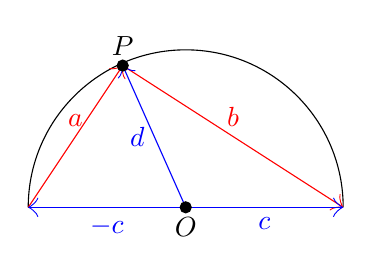
\begin{tikzpicture}
                    \draw (2,0) arc (0:180:2cm);
                    \draw (-2,0) -- (2,0);
                    \draw[-{Classical TikZ Rightarrow[scale=2]},color=red] (-2,0) -- (-0.8,1.8) node[midway,above] {$\vv a$};
                    \draw[-{Classical TikZ Rightarrow[scale=2]},color=red] (-0.8,1.8) -- (2,0) node[midway,above] {$\vv b$};
                    \draw[-{Classical TikZ Rightarrow[scale=2]},color=blue] (0,0) -- (2,0) node[midway,below] {$\vv c$};
                    \draw[-{Classical TikZ Rightarrow[scale=2]},color=blue] (0,0) -- (-2,0) node[midway,below] {$-\vv c$};
                    \draw[-{Classical TikZ Rightarrow[scale=2]},color=blue] (0,0) -- (-0.8,1.8) node[midway,left] {$\vv d$};
                    \draw[fill] (0,0) circle (2pt) node[below] {$O$};
                    \draw[fill] (-0.8,1.8) circle (2pt) node[above] {$P$};
                \end{tikzpicture}
            \end{center}
            By properties of vector addition,
            $$
            \vv d + \vv b = \vv c \qquad -\vv c + \vv a = \vv d
            $$
            Rearrange
            $$
            \vv b = \vv c - \vv d \qquad \vv a = \vv d + \vv c
            $$
            Take the dot product between $\vv a$ and $\vv b$
            \begin{align*}
                \vv a \cdot \vv b &= (\vv c + \vv d) \cdot (\vv c - \vv d) \\
                &= \vv c \cdot \vv c - \vv d \cdot \vv d \\
                &= \norm{c}^2 - \norm{d}^2
            \end{align*}
            Since both $\vv c$ and $\vv d$ are the radii of the circle, $\norm{c}=\norm{d}=r$ where $r$ is the radius of the circle. Then,
            $$
            \vv a \cdot \vv b = \norm{c}^2 - \norm{d}^2 = 0
            $$
            This implies that $\vv a$ is orthogonal to $\vv b$.
        \end{proof}
        
        \item
        \begin{proof}
            \hfill \\
            Geometrically, consider the following half circle.
            \begin{center}
                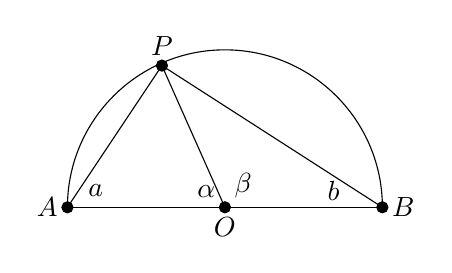
\begin{tikzpicture}
                    \draw (2,0) arc (0:180:2cm);
                    \draw (-2,0) -- (2,0);
                    \draw (-2,0) -- (-0.8,1.8);
                    \draw (-0.8,1.8) -- (2,0);
                    \draw (0,0) -- (-0.8,1.8);
                    \draw[fill] (0,0) circle (2pt) node[below] {$O$};
                    \draw[fill] (-0.8,1.8) circle (2pt) node[above] {$P$};
                    \draw[fill] (-2,0) circle (2pt) node[left] {$A$};
                    \draw[fill] (2,0) circle (2pt) node[right] {$B$};
                    \node[above left] at (0,0) {$\alpha$};
                    \node[above right] at (0,0) {$\beta$};
                    \node[above=6pt, right=4pt] at (-2,0) {$a$};
                    \node[above=6pt, left=12pt] at (2,0) {$b$};
                \end{tikzpicture}
            \end{center}
            In a circle, $OA=OP=r$ where $r$ is the radius. Hence, $\triangle OPA$ is an isosceles triangle, which implies that $\angle OAP = \angle OPA = a$. Similarly, $\angle OBP = \angle OPB = b$.
            
            Since the sum of internal angles for a triangle is $180\degree$, $2a+\alpha = 180\degree$ and $2b+\beta = 180\degree$.
            
            Additionally, $\alpha + \beta = 180\degree$. So, $\alpha + \beta = 360\degree - 2a - 2b$.
            \begin{align*}
                \alpha + \beta &= 360\degree - 2(a+b) \\
                180\degree &= 360\degree - 2(a+b) \\
                2(a+b) &= 180\degree \\
                a+b &= 90\degree
            \end{align*}
            Hence, $\angle APB = \angle OPA + \angle OPB = a+b = 90\degree$.
        \end{proof}
    \end{enumerate}
    
    \item Question 12
    
    \item Question 13
    
    \begin{proof}
    \hfill \\
    Assume $\vv{A}=\vv{A_1}+\vv{A_2}$ and $\vv{A_1}\cdot \vv{B}$. And $\vv{A_2}$ is parallel to $\vv{B}$. This implies that there exists some $k\in\R$ such that $\vv{A_2} = k\vv{B}$.
    
    Let $\theta$ be the angle between $\vv{A_2}$ and $\vv{B}$. Since the two vectors are parallel, $\theta=0$ and $\cos\theta=1$. By property of the dot product, 
    $$
    \vv{A_2}\cdot\vv{B}=\norm{\vv{A_2}}\norm{\vv{B}}\cos\theta = \norm{\vv{A_2}}\norm{\vv{B}}
    $$
    Since $\vv{A}=\vv{A_1}+\vv{A_2}$ and $\vv{A_2} = k\vv{B}$, then $\vv{A}=\vv{A_1}+k\vv{B}$. It follows that $\vv{A_1}=\vv{A}-k\vv{B}$ by vector algebra.
    
    Since $\vv{A_1}\cdot\vv{B}=0$,
    \begin{align*}
        (\vv{A}-k\vv{B})\cdot \vv{B} &= 0 \\
        \vv{A}\cdot\vv{B}-k\vv{B}\cdot\vv{B} &= 0  & \text{by distributive property}\\
        \vv{A}\cdot\vv{B} &= k\vv{B}\cdot\vv{B} \\
        k &= \frac{\vv{A}\cdot\vv{B}}{\vv{B}\cdot\vv{B}}
    \end{align*}
    Since $\vv{A_2} = k\vv{B}$,
    $$
    \vv{A_2} = \frac{\vv{A}\cdot\vv{B}}{\vv{B}\cdot\vv{B}} \cdot \vv{B}
    $$
    \end{proof}
    
    \item Question 14
    
    \item Question 15
    \begin{enumerate}
        \item     
        \begin{align*}
            \norm{\vv A - t\vv B}^2 &= (\vv A - t\vv B)\cdot (\vv A - t \vv B) \\
            &= \vv A \cdot \vv A - t\vv A \cdot \vv B - t \vv A \cdot \vv B + t^2\vv B \cdot \vv B \\
            &= \norm{\vv A}^2 -2t(\vv A \cdot \vv B) + \norm{\vv B}^2t^2
        \end{align*}
        
        \item
        \hfill
        \begin{proof}
            \hfill \\
            Let $A$ and $B$ be arbitrary vectors.
            Define $P(t)=\norm{A}-2t(A\cdot B)+\norm{B}^2t^2 = (\norm{A-tB})^2$
            
            $P(t)$ will always be non-negative. Then, $P(t)=0$ has one or no solution.
            
            This implies that the discriminant $\Delta \leq 0$.
            
            By definition of the discriminant
            \begin{align*}
                \Delta = (-2(A \cdot B))^2 -4 \norm{B}^2 \norm{A}^2 &\leq 0 \\
                4(A\cdot B)^2 &\leq 4 \norm{A}^2\norm{B}^2 \\
                \sqrt{(A\cdot B)^2} & \leq \sqrt{\norm{A}^2\norm{B}^2}
            \end{align*}
            We can take out the square root. Hence, $|A\cdot B| \leq \norm{A}\norm{B}$.
            
            By generalization, for all vectors, the Cauchy-Schwartz Inequality holds.
        \end{proof}
    \end{enumerate}
    
    \item Question 16
    \hfill
    \begin{proof}
        \hfill \\
        Let $\vv u$ and $\vv v$ be arbitrary.
        
        By property of vector arithmetic,
        \begin{align*}
            \norm{\vv u + \vv v}^2 &= (\vv u + \vv v)\cdot (\vv u + \vv v) \\
            &= \vv u \cdot \vv v + 2\vv u \cdot \vv v + \vv v \cdot \vv v \\
            &= \norm{\vv u}^2 + 2(\vv u \cdot \vv v) + \norm{\vv v}^2
        \end{align*}

        By property of absolute value,
        $$
        \norm{\vv u}^2 + 2(\vv u \cdot \vv v) + \norm{\vv v}^2 \leq \norm{\vv u}^2 + 2 |\vv u \cdot \vv v| + \norm{\vv v}^2
        $$
        By Cauchy-Schwartz Inequality
        $$
        \norm{\vv u}^2 + 2 |\vv u \cdot \vv v| + \norm{\vv v}^2 \leq \norm{\vv u}^2 + 2 \norm{\vv u}\norm{\vv v} + \norm{\vv v}^2
        $$
        Then,
        $$
        \norm{\vv u + \vv v}^2 \leq (\norm{\vv u}+\norm{\vv v})
        $$
        Taking square root of both side gives
        $$
        \norm{\vv u + \vv v} \leq \norm{\vv u} + \norm{\vv v}
        $$
        By generalization, for all vectors $\vv u$ and $\vv v$, the Triangle Inequality holds.
    \end{proof}
    
    \item Question 17
    
    \item Question 18
    
    \item Question 19
    
    \item Question 20
\end{enumerate}

\end{document}